\documentclass{article}
\usepackage{mathtools, blkarray}
\usepackage{graphics,graphicx}
\usepackage{tikz}

\usetikzlibrary{arrows,snakes,backgrounds}



\makeatletter
% we use \prefix@<level> only if it is defined
\renewcommand{\@seccntformat}[1]{%
  \ifcsname prefix@#1\endcsname
    \csname prefix@#1\endcsname
  \else
    \csname the#1\endcsname\quad
  \fi}
% define \prefix@subsection
\newcommand\prefix@subsection{}
\makeatother

\makeatletter
% we use \prefix@<level> only if it is defined
\renewcommand{\@seccntformat}[1]{%
  \ifcsname prefix@#1\endcsname
    \csname prefix@#1\endcsname
  \else
    \csname the#1\endcsname\quad
  \fi}
% define \prefix@subsubsection
\newcommand\prefix@subsubsection{ }
\makeatother

\newcommand{\mytilde}{\raise.17ex\hbox{$\scriptstyle\mathtt{\sim}$}}


\begin{document}

\title{Math 775: Homework 3}
\author{Alex Dewey}


\maketitle


\section{Notes}

Make all the figures smaller.

2.11. Redo as three figures.

2.13. Start

3.1. Review proof

3.2. Rewrite

3.3. Done

3.4. Done

Pt II

1. Decide on strategy, finish, write-up.

2. Add plots.

3. Look up gamma with known rate, review normal?

4. Add plots

\section{Exercises}

\subsection{Chapter 2 - Problem 11.}

The histograms are below.

\begin{figure}[!ht]
  \centering
   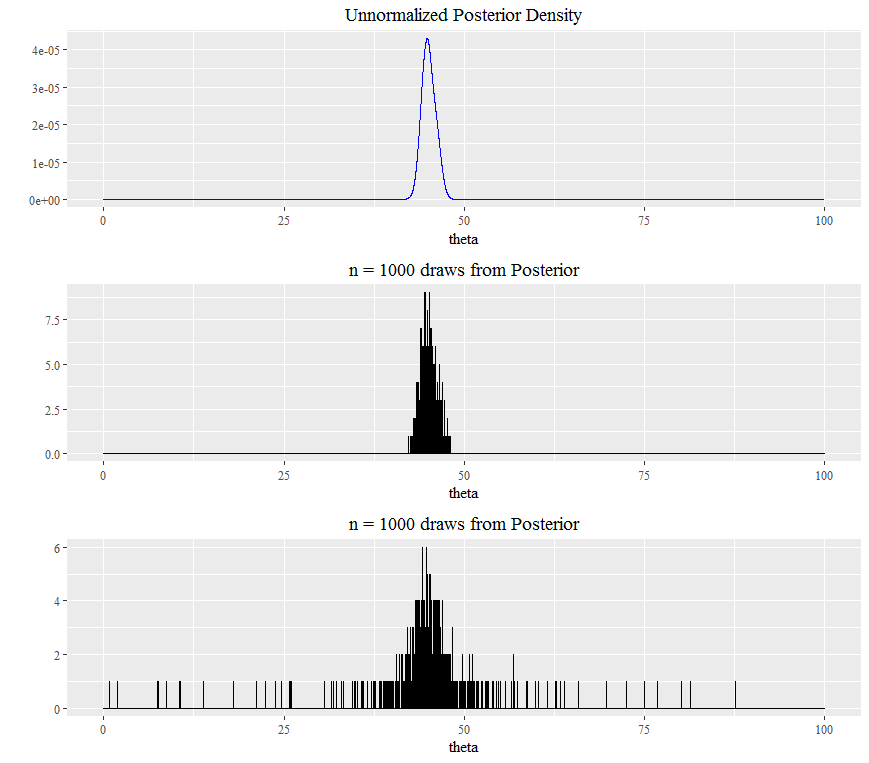
\includegraphics[width=\textwidth]{Problem211-1}
   \caption{Top: The unnormalized posterior \(\theta \vert y\).}
  \caption{Middle: 1000 draws from this posterior.}
  \caption{Bottom: Predictive posterior samples, each conditioned on one of the 1000 draws above.
  \(p(\tilde{y} \vert \theta, y)\).}
\end{figure}

\subsection{Chapter 2 - Problem 13.}

Let's use a gamma prior representing 3 years of data with 20 fatal accidents each.

\(p(\theta) = \Gamma(60, 3)\)
\(p(y \vert \theta) = {\theta^k e^{-\theta} \over k!}\)

\subsection{Chapter 3 - Problem 1.}

First, assume that \(y = (y_1, y_2, ..., y_J)\) follows a normal distribution and that
 \(\theta = (\theta_1, \theta_2, ..., \theta_J)\) has a Dirichlet prior with parameters
 \(\beta = (\beta_1, \beta_2, ..., \beta_J)\).
 
So our prior is \(p(\theta) \propto \prod_{j=1}^J \theta_j^{\beta_j - 1}\)
 and our sampling distribution is \(p(y \vert \theta) \propto \prod_{j=1}^J \theta_j^{y_j}\).

Therefore our unnormalized joint posterior is
\(p(\theta \vert y) \propto \prod_{j=1}^J \theta_j^{y_j + \beta_j - 1}\),
a Dirichlet with parameters \(\beta_j + y_j\).

Consider a uniform (\(u = (u_1, u_2, ..., u_n) \mytilde U_{[0,1]}\)) 
sampling scheme from the joint posterior 
which rejects drawn values if \(u_i > \theta_1 + \theta_2\),
and then takes on a value of \(x_{u_i} = 1\) if \(u_i \leq \theta_1\) and \(x_{u_i} = 0\) otherwise (assuming \(u_i\) was accepted). 

So each \(x_i\) is a Bernoulli trial with parameter
\({\theta_1 \over \theta_1 + \theta_2} = \alpha\).

Let k be the number of accepted values in our sample. Note that k = \(y_1 + y_2\), 
\(\sum x_j = y_1\), and thus \(k - \sum x_j = y_2\)  . 

By definition, then, our sampling distribution is \[p(x \vert \theta, k) \propto \alpha^{\sum x_j} (1 - \alpha)^{k - \sum x_j} = \alpha^{y_1} (1 - \alpha)^{y_2}\]. This is a binomial distribution,
and if we treat the first two elements of our prior \((\beta_1, \beta_2)\) as parameters for
our (conjugate) beta prior, we derive a beta posterior with parameters 
\((\beta_1 + y_1, \beta_2 + y_2)\).

In other words, we can use rejection sampling (implicitly or not) to get a separate, consistent beta-binomial model by looking only at the first two parameters, and 
\(\alpha \vert y \mytilde Beta(\beta_1 + y_1, \beta_2 + y_2)\).

\subsection{Chapter 3 - Problem 2.}

Let's ignore the third data category (``No opinion/other'') through the result in Problem 3.1 above, which says that we can effectively
look at the respective proportions in the first two categories (``Bush, Dukakis'') as coming from beta-binomial model. The only subtlety with that is to treat the respective sample sizes in this model as 601, 620, not as 639 each. Suppose our beta prior is \(Beta(1,1)\) (though this doesn't really matter with such sample sizes). Then we get two beta posteriors--the pre-debate posterior is \(\alpha_1 \vert y \mytilde Beta(295, 308)\) and the post-debate posterior is \(\alpha_2 \vert y \mytilde Beta(289, 333)\).

This is probably not too difficult analytically, given that we're taking the linear difference of two estimands which have simple, well-known distributions. But even more easily, we could successively sample a bunch of times from each distribution and look at the difference. Also, in order to avoid overcomplicating things, it's natural to produce a paired sample for each trial--so for each trial we sample a proportion from the pre-debate posterior and another from the post-debate posterior, and look at the paired difference of the experiment. Below is the histogram for 1,000 such trials.

\begin{figure}[!ht]
  \caption{The distribution of \(\alpha_{post} - \alpha_{pre}\) in n=10,000 posterior samples.}
  \centering
    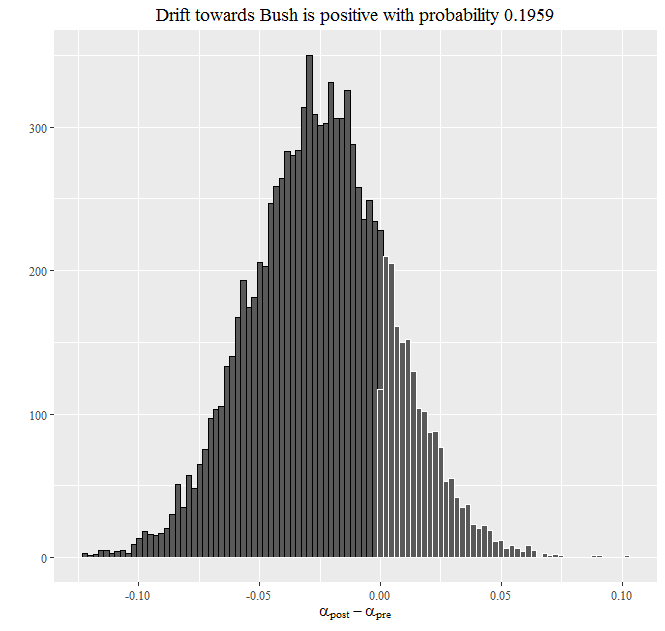
\includegraphics[width=\textwidth]{Problem32--Debate}
\end{figure}


\subsection{Chapter 3 - Problem 3.}

From the derivation in the book of a normal with the non-informative uniform prior 
on \( (\mu_c, \mu_t, \log \sigma_c, \log \sigma_t)\), we know that the sample mean and standard
deviation are sufficient statistics in the t-distribution that \(\mu\) follows:

\[ \mu \vert y \mytilde t_{n-1}(\bar{y}, s^2/n)\]. 

For the control group of chickens, we have
\( \mu_c \vert y \mytilde t_{31}(1.013, (0.24^2)/32)\). For the treatment group, we have
\( \mu_t \vert y \mytilde t_{35}(1.173, (0.20^2)/36)\).

The posterior sampling from these distribution turns out to be easier if one generates t values
and then adjusts them by multiplying by \(s / \sqrt{n}\), then adding \(\bar{y}\). Below is the histogram of 10,000 trials.

\begin{figure}[!ht]
  \caption{The distribution of calcium flow increases in n=10,000 posterior samples.}
  \centering
    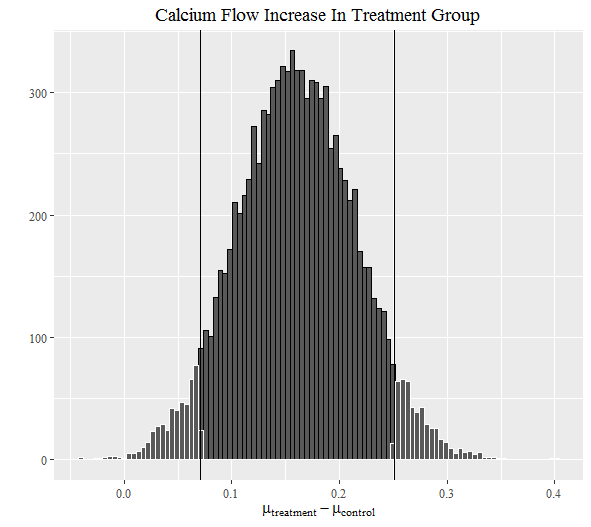
\includegraphics[width=\textwidth]{HW3--Problem33}
\end{figure}


\subsection{Chapter 3 - Problem 4.}

I used the noninformative prior \(Beta(1,1)\) for each group and so the posteriors
were \(Beta(636, 40)\) for the control and \(Beta(659, 23)\) for the treatment.

Below are histograms of 10,000 posterior draws from the control group, the treatment group,
and the odds ratio, showing that the data strongly favors the treatment group.

This inference is highly sensitive to the prior--I chose a perfunctory noninformative prior, but if I'd changed the strength of the prior to, say, \(Beta(10,10)\) the posterior mortality rate under the control would increase by around 25\% and the posterior mortality rate under treatment would increase by around 40\%. So it would clearly make a difference to the inference.

Also, with life-expectancy data, it may be possible to estimate the expected mortality rates of each of the patients (or a mixture distribution from different levels of mortality risk) to make the model more sophisticated.

\begin{figure}[!ht]
  \caption{Control}
  \centering
    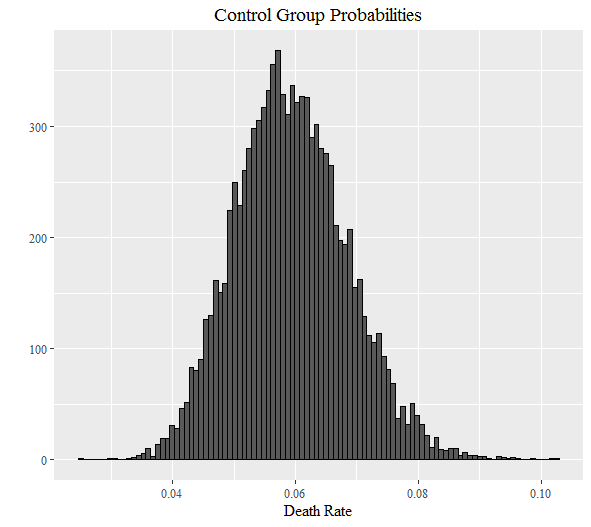
\includegraphics[width=\textwidth]{Problem34--Control}
\end{figure}

\begin{figure}[!ht]
  \caption{Treatment}
  \centering
    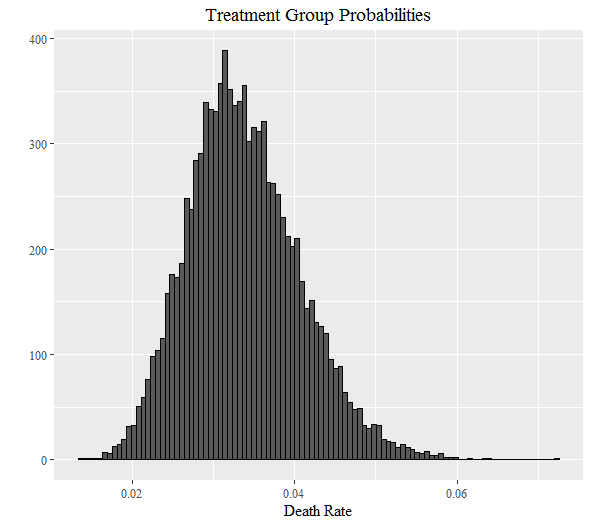
\includegraphics[width=\textwidth]{Problem34--Treatment}
\end{figure}

\begin{figure}[!ht]
  \caption{Odds}
  \centering
    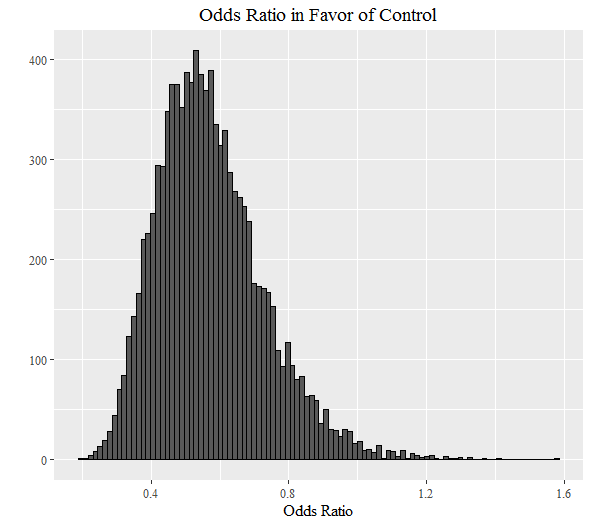
\includegraphics[width=\textwidth]{Problem34--Odds}
\end{figure}

\subsection{Exercise 1.}

Vector argument--metric distance.

denominator \(\sum_i (y_i - \bar{y})^2\) is sample variance. Rewrite minus sign to plus
sign to see that if coefficient of \(y_i - \bar{y}\) is equal to 1, then \(\hat{\theta_i}(y) = \bar{y}\)

\(\theta_i\) is the population parameter \(y_i\) is the sample. \(E_y\sum (y_i - \theta_i)^2\) is just
chi-squared with m df and hence its expected value is m.

Maybe try showing that the expectation of \(\hat{\theta_i} - \theta_i\) for all i.

Nothing depends on the magnitude of \(\theta_i\) so might as well assume they're 0


\subsection{Exercise 2.}

\subsubsection{a.}

By integrating \(g(y) = e^{-y}\) from 0 to \(\infty\), we easily obtain the CDF \(G(y) = 1 - e^{-y}\).
So we generate \(u \mytilde U_{[0,1]}\), set \(G(y) = u\) and try to derive y by inverting the CDF. 

Since a uniform variable from 0 to 1 is the same as a uniform variable from 1 to 0, we might as well
say \(u = e^{-y}\), and from this, we can easily derive \(y = -\log{u}\). 

So we generate a uniform random variable u,
take its logarithm (which is guaranteed to be negative), negate it, and use the output as our generated 
value for y, and we should have \(y \mytilde g(y) = e^{-y}\). 

\subsubsection{b.}

Integrating the Weibull distribution is made much simpler by noting that for nonzero a we have \({dy^a \over dy} = ay^{a - 1}\).

So we're integrating over the same exponential PDF \(\int e^{-v}dv\) as we did in (a), over the same domain,
but with the substitution \(v = y^3\).

Evaluating the antiderivative and substituting \(v = y^3\) back in, 
we get the CDF  \(G(y) = 1 - e^{-y^3}\). Inverting this function
is similar to (a), with \(y = (-\log{u})^{1/3}\).

\subsubsection{c.}

This integral is very difficult without noticing that the Cauchy function \(g(y) = {1 \over \pi (1 + y^2)}\) is just the scaled derivative
of the arctangent function. Because the domain of the tangent function (for the purposes of a bijection)
is over \([-\pi/2, \pi/2]\) we have to shift our uniform variable u into this domain
before taking its tangent. By taking \(y = \tan{\pi*(u - 1/2)}\) we can generate y according to a Cauchy distribtuion.

\subsubsection{d.}

The integral of the F distribution looks much more difficult than it is--most of the multiplicative terms
are constants of integration, and what's left is a polynomial function \(g(y) \propto y(1 + 2y/3)^{-5}\).
This PDF is most easily integrated by taking the substitution \(v = 1 + 2y/3\). After some algebra (including
multiplying by a term of \(u^4)\)), the inverse-CDF
works out to be the root exceeding 1 of the quartic polynomial \(u*v^4 - 4*v + 3 = 0\).
for our uniform variable u, which I computed with Newton's method and a seed value of 20.

Finally, I undo the substitution \(3/2(v - 1)= y\).




\subsection{Exercise 3.}



\subsubsection{i.}

For the negative binomial, any given outcome represents y successes and r failures (after which
the trial ends).
With the likelihood given (\(P(y\vert \theta) = {y + r - 1 \choose y}\theta^r, (1 - \theta)^y\)), 
\(\theta\) represents the probability of failure.
So a natural prior would be a distribution representing
\(\alpha\) failures and \(\beta\) successes in the parameter \(\theta\).

A natural way to do this is with the beta function having parameters \((\alpha, \beta)\), so 
that the posterior has a beta function with parameters \((\alpha + r, \beta + y)\).

Formally, \(p(\theta) \propto \theta^{\alpha - 1}(1 - \theta)^{\beta - 1}\) and
\(p(\theta \vert y) \propto \theta^{\alpha + r - 1}(1 - \theta)^{\beta + y - 1}\)

\subsubsection{ii.}
\subsubsection{iii.}
\subsubsection{iv.}


\end{document}